The parallelization strategy we have chosen to use on clusters is \emph{Root parallelization}.
\emph{Root parallelization} consists in giving the tree that we want to develop to every actor (here each machine is an actor), letting them develop it randomly without any communication with the environment during a certain amount of time, and then merging the results of each tree.
It is depicted in figure \ref{fig:root}.
This method has the great benefit of minimizing the communication between the machines, as they only communicate at the beginning and at the end of the algorithm, without needing any further synchronization.

\begin{figure}[!ht] 
\centerline{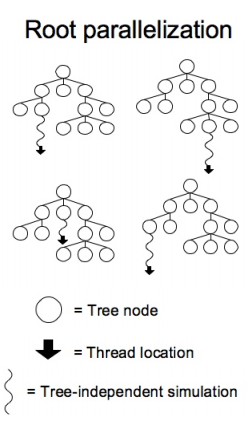
\includegraphics[scale=0.5]{Parallelisation/Strategy/Img/root.png}}
   \caption{Overview of \emph{Root Parallelization} \cite{parallel_comp}}
\label{fig:root}
\end{figure}

In order to apply this strategy, we have chosen a master-slave approach, with one master machine collecting the results of every other machine once they are done with their processing.
The algorithm will proceed as follows :
\begin{itemize}
	\item The master will asynchronously send the state of the game to the slaves
	\item The slaves will get the state of the game sent by the master with blocking receive requests
	\item Every machine will run its simulations by itself, building its own tree
	\item At regular intervals, each slave will asynchronously send messages with the current state of its tree
	\item The master will then receive these messages with asynchronous receive requests, and update its own tree with their results
	\item At the end of the given time, the master will process the best move with the help of its tree
\end{itemize}

The \emph{Message Passing Interface Standard} (\emph{MPI}) is a message passing library standard.
We plan to use it for machine parallelization if the tests give satisfying results.
In order to make the different machines communicate, it opens ssh connexions between them.
The general structure of a MPI program can be seen in figure \ref{fig:mpi_struct}.

\begin{figure}[H]
\centering
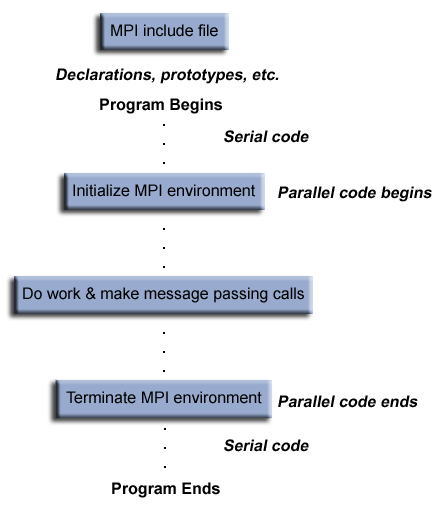
\includegraphics[width=.5\textwidth]{Parallelisation/Cluster/Img/prog_structure.png}
\caption{General MPI Program Structure. \cite{mpi_tuto}}
\label{fig:mpi_struct}
\end{figure}

MPI uses objects called communicators and groups to define which collection of processes may communicate with each other.
Within a communicator, every process has its own unique, integer identifier assigned by the system when the process initializes.
These ranks are used by the programmer to specify the source and destination of messages.

MPI allows for synchronized, blocking and non blocking routines.
Synchronized sending requests only return after the message has been received, while blocking ones return after it is safe to modify the data in the sending buffer, and non blocking ones return immediately after sending the order, but offer no guarantee that it has already been executed.

Another type of routines handled by MPI is Collective Communication Routines.
They allow to make a similar operation on every process of a given communicator.
For example, it is possible to spread data from a single process to each other process, or on the contrary to regroup data from every process into a single one (as represented in figure \ref{fig:mpi_ccr}), where all the data is gathered in task 1).
This will be especially useful for the algorithm, as it will require to regroup the results of every process.

\begin{figure}[H]
\centering
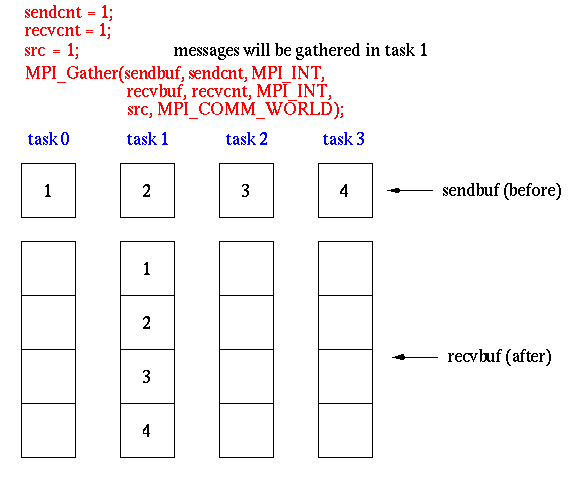
\includegraphics[width=.6\textwidth]{Parallelisation/Cluster/Img/MPI_Gather.png}
\caption[Example of a Collective Communication Routine (\cite{mpi_tuto}). ]{Example of a Collective Communication Routine (\cite{mpi_tuto}). Here we can see task 1 gathering the data from every other task.}
\label{fig:mpi_ccr}
\end{figure}